\documentclass[10pt,a4paper]{ctexart}
\usepackage[margin=2cm]{geometry}
\usepackage{graphicx}
\usepackage{float}      % 支持 [H] 浮动体选项
\usepackage{hyperref}
\usepackage{amsmath}    % 提供方程环境
\usepackage{physics}    % 简化向量、微分算子语法
\newcommand{\myspace}[1]{\par\vspace{#1\baselineskip}} %自定义空一行
\usepackage{fancyhdr}
\usepackage{tabularx}
\pagestyle{fancy}
\fancyhf{}  % 清除所有页眉页脚
\fancyfoot[C]{\thepage}  % 在页脚中央设置页码
\renewcommand{\headrulewidth}{0pt}  % 去掉页眉横线
\renewcommand{\footrulewidth}{0pt}  % 去掉页脚横线

\usepackage{hyperref}
\hypersetup{
    colorlinks=true,
    linkcolor=blue,
    filecolor=magenta,      
    urlcolor=cyan,
    pdftitle={Overleaf Example},
    pdfpagemode=FullScreen,
    }

\usepackage{titlesec}

% 重新定义section格式
\titleformat{\section}
  {\normalfont\Large\bfseries}
  {\chinese{section}、}
  {0pt}
  {}

% 给出常用字号的自定义指令
\newcommand{\chuhao}{\fontsize{42pt}{48pt}\selectfont}
\newcommand{\xiaochu}{\fontsize{36pt}{42pt}\selectfont}
\newcommand{\xiaoer}{\fontsize{18pt}{21.6pt}\selectfont}
\newcommand{\sanhao}{\fontsize{16pt}{20pt}\selectfont}
\newcommand{\xiaosan}{\fontsize{15pt}{18pt}\selectfont}
\newcommand{\sihao}{\fontsize{14pt}{18pt}\selectfont}
\newcommand{\xiaosi}{\fontsize{12pt}{16pt}\selectfont}
\newcommand{\wuhao}{\fontsize{10.5pt}{12.6pt}\selectfont}

% 定义中文数字转换
\titleformat{\section}
  {\normalfont\Large\bfseries}
  {\zhnum{section}、}  % 使用\zhnum而不是\chinese
  {0pt}
  {}

% 标题设置
\title{\xiaochu\textbf{物理实验报告}}
\author{}
\date{}

\begin{document}

\vspace*{36pt} % 顶部空白

% 居中填写区域
\begin{center}
    
\includegraphics[width = 9cm]{figure/head.png}
    
    \xiaochu\textbf{物理实验报告}
    % 预留空白区域
    \vspace{13pt}
    \vspace{13pt}
    \vspace{13pt}
    \vspace{13pt}
    
    \sanhao\textbf{实验名称：\underline{\makebox[10cm]{ 非平衡电桥}}} \\[10pt]
    \sanhao\textbf{实验桌号：\underline{\makebox[10cm]{ 10}}} \\[10pt]
    \sanhao\textbf{指导教师：\underline{\makebox[10cm]{ 唐浩原 }}} \\[30pt]
    
    % 预留空白区域
    \myspace{6}
    
   \sihao\textbf{班级：\underline{\makebox[6cm]{}}} \\[10pt]
    \sihao\textbf{姓名：\underline{\makebox[6cm]{}}} \\[10pt]
    \sihao\textbf{学号：\underline{\makebox[6cm]{}}} \\[30pt]
    
   \sihao\textbf{实验日期: 
   \underline{\makebox[0.8cm]{2025}}  年 
   \underline{\makebox[0.4cm]{11}}月
   \underline{\makebox[0.4cm]{19}}日  
   星期\underline{\makebox[0.6cm]{三}}上午}
    
    \vspace{18pt}
    \sihao 浙江大学物理实验教学中心
    
\end{center}

\newpage

\section{预习报告}

    \subsection{实验综述}
    
    \xiaosi （自述实验现象、实验原理和实验方法，不超过300字，5分）
 
     非平衡电桥测量温度系数时，电桥非平衡状态下会输出电压U，而电阻会随温度变化，导致电压也随温度变化，
    在$R_1=R_2=R_3=R_0$时($R_0$表示待测电阻在0℃时的阻值)电压和温度系数具有定量关系
    \[
        U=\frac{\alpha t}{4+2 \alpha t}E
    \]
    通过测量不同温度下的电压U，可以计算出待测电阻的温度系数$\alpha$。

    平衡电桥法测量温度系数通过调节电桥平衡测量电阻，同时记录此时温度，拟合温度与电阻的关系曲线，计算温度系数$\alpha$。
    
     \myspace{2}
    \subsection{实验重点}
    
    \xiaosi（简述本实验的学习重点，不超过100字，3分）
    
1. 掌握非平衡电桥的工作原理和测量方法


2. 理解温度系数与电阻变化的关系

3. 学会通过电压测量计算温度系数

4. 掌握平衡电桥法测量电阻温度特性的方法
    \myspace{2}
    
    \subsection{实验难点}
    
    \xiaosi（简述本实验的实现难点，不超过100字，2分）

1. 准确控制和测量温度

2. 电桥平衡点的精确判断

3. 电压信号的准确测量

4. 温度系数计算中的误差分析

5. 数据拟合与结果验证

6.电阻值准确调整
\myspace{2}
\section{原始数据}

    \xiaosi （将有老师签名的“自备数据记录草稿纸”的扫描或手机拍摄图粘贴在下方，20分）
   
\begin{figure}[H]
    \centering
    
\includegraphics[width=0.9\textwidth]{figure/raw_data.jpg}
    \caption{非平衡电桥原始数据记录}
\end{figure}
\section{结果与分析}

    \subsection{数据处理与结果}
    \xiaosi （列出数据表格、选择数据处理方法、给定测量或计算结果，30分）

    保持电源电压E=1.3V不变，$R_1=R_2=R_3=R_0=50.00\Omega$，改变温度测量电压，使用非平衡电桥法测量温度系数，记录数据如下表所示：
    \begin{table}[H]
\centering
\caption{非平衡电桥测温度系数数据记录表}
\vspace{2mm}
{\small \centering 实验条件：E = 1.3\,V \quad; \quad $\alpha_{\mathrm{theory}}=4.28 \times 10^{-3}$ \par}
\vspace{2mm}
\begin{tabularx}{0.9\textwidth}{>{\centering\arraybackslash}m{0.2\textwidth}|*{8}{>{\centering\arraybackslash}X}}
\hline
次序 & 1 & 2 & 3 & 4 & 5 & 6 & 7 & 8 \\
\hline
温度 $t/^{\circ}\mathrm{C}$ &16.5 &21.6 &25.9 &30.6 &35.0 &39.8 &44.7 &49.4 \\
\hline
 $U$/mV &22.5 &29.2 &34.0 &40.0 &45.5 &51.1 &56.8 &62.5 \\
\hline
温度系数 $\alpha$/$\left(10^{-3}\,^{\circ}\mathrm{C}^{-1}\right)$ & $4.03$ & $4.01$ & $4.05$ & $4.07$ & $4.07$ & $4.10$ & $4.11$ & $4.12$ \\
\hline
\end{tabularx}
\end{table}
由表根据公式
\begin{equation}
    \alpha=\frac{4 U}{t(E-2 U)}
\end{equation}
其中E=1.3V，计算出各温度下的温度系数$\alpha$，计算结果如上表所示。取各次测量结果的平均值，得到非平衡电桥测得的温度系数为
\[
    \alpha_{\mathrm{non\text{-}balance}}= 4.07\times10^{-3}\,^{\circ}\mathrm{C}^{-1}
\]
相对误差为
\[
    \delta_{\mathrm{non\text{-}balance}}=\left|\frac{\alpha_{\mathrm{non\text{-}balance}}-\alpha_{\mathrm{theory}}}{\alpha_{\mathrm{theory}}}\right|=5.0\%
\]
接下来使用平衡电桥法测量温度系数，保持$R_1=R_2$，调节$R_3$，当电压为0V时读出$R_3$阻值，记录数据如下表所示：

\begin{table}[H]
\centering
\caption{平衡电桥测温度特性数据记录表}
\vspace{2mm}
{\small \centering 实验条件：E = 1.3\,V \quad; \quad $\alpha_{\mathrm{theory}}=0.00428$ \par}
\vspace{2mm}
\begin{tabularx}{0.9\textwidth}{>{\centering\arraybackslash}p{0.2\textwidth}|*{8}{>{\centering\arraybackslash}X}}
\hline
次序 & 1 & 2 & 3 & 4 & 5 & 6 & 7 & 8 \\
\hline
温度 $t/^{\circ}\mathrm{C}$ &16.5 &21.6 &25.9 &30.6 &35.0 &39.8 &44.7 &49.7 \\
\hline
$R_t/\Omega$ &54.02 &55.09 &56.06 &56.86 &58.01 &59.00 &60.07 &61.10 \\
\hline
\end{tabularx}
\end{table}
根据上表的数据，对 $R_t$ 与 $t$ 进行最小二乘线性拟合：得到 $R(t)=R_0(1+\alpha t)$，其中 $R_0=50.00\Omega$，$\alpha=4.29\times10^{-3}\,^{\circ}\mathrm{C}^{-1}$。
拟合曲线如下
\begin{figure}[H]
    \centering
    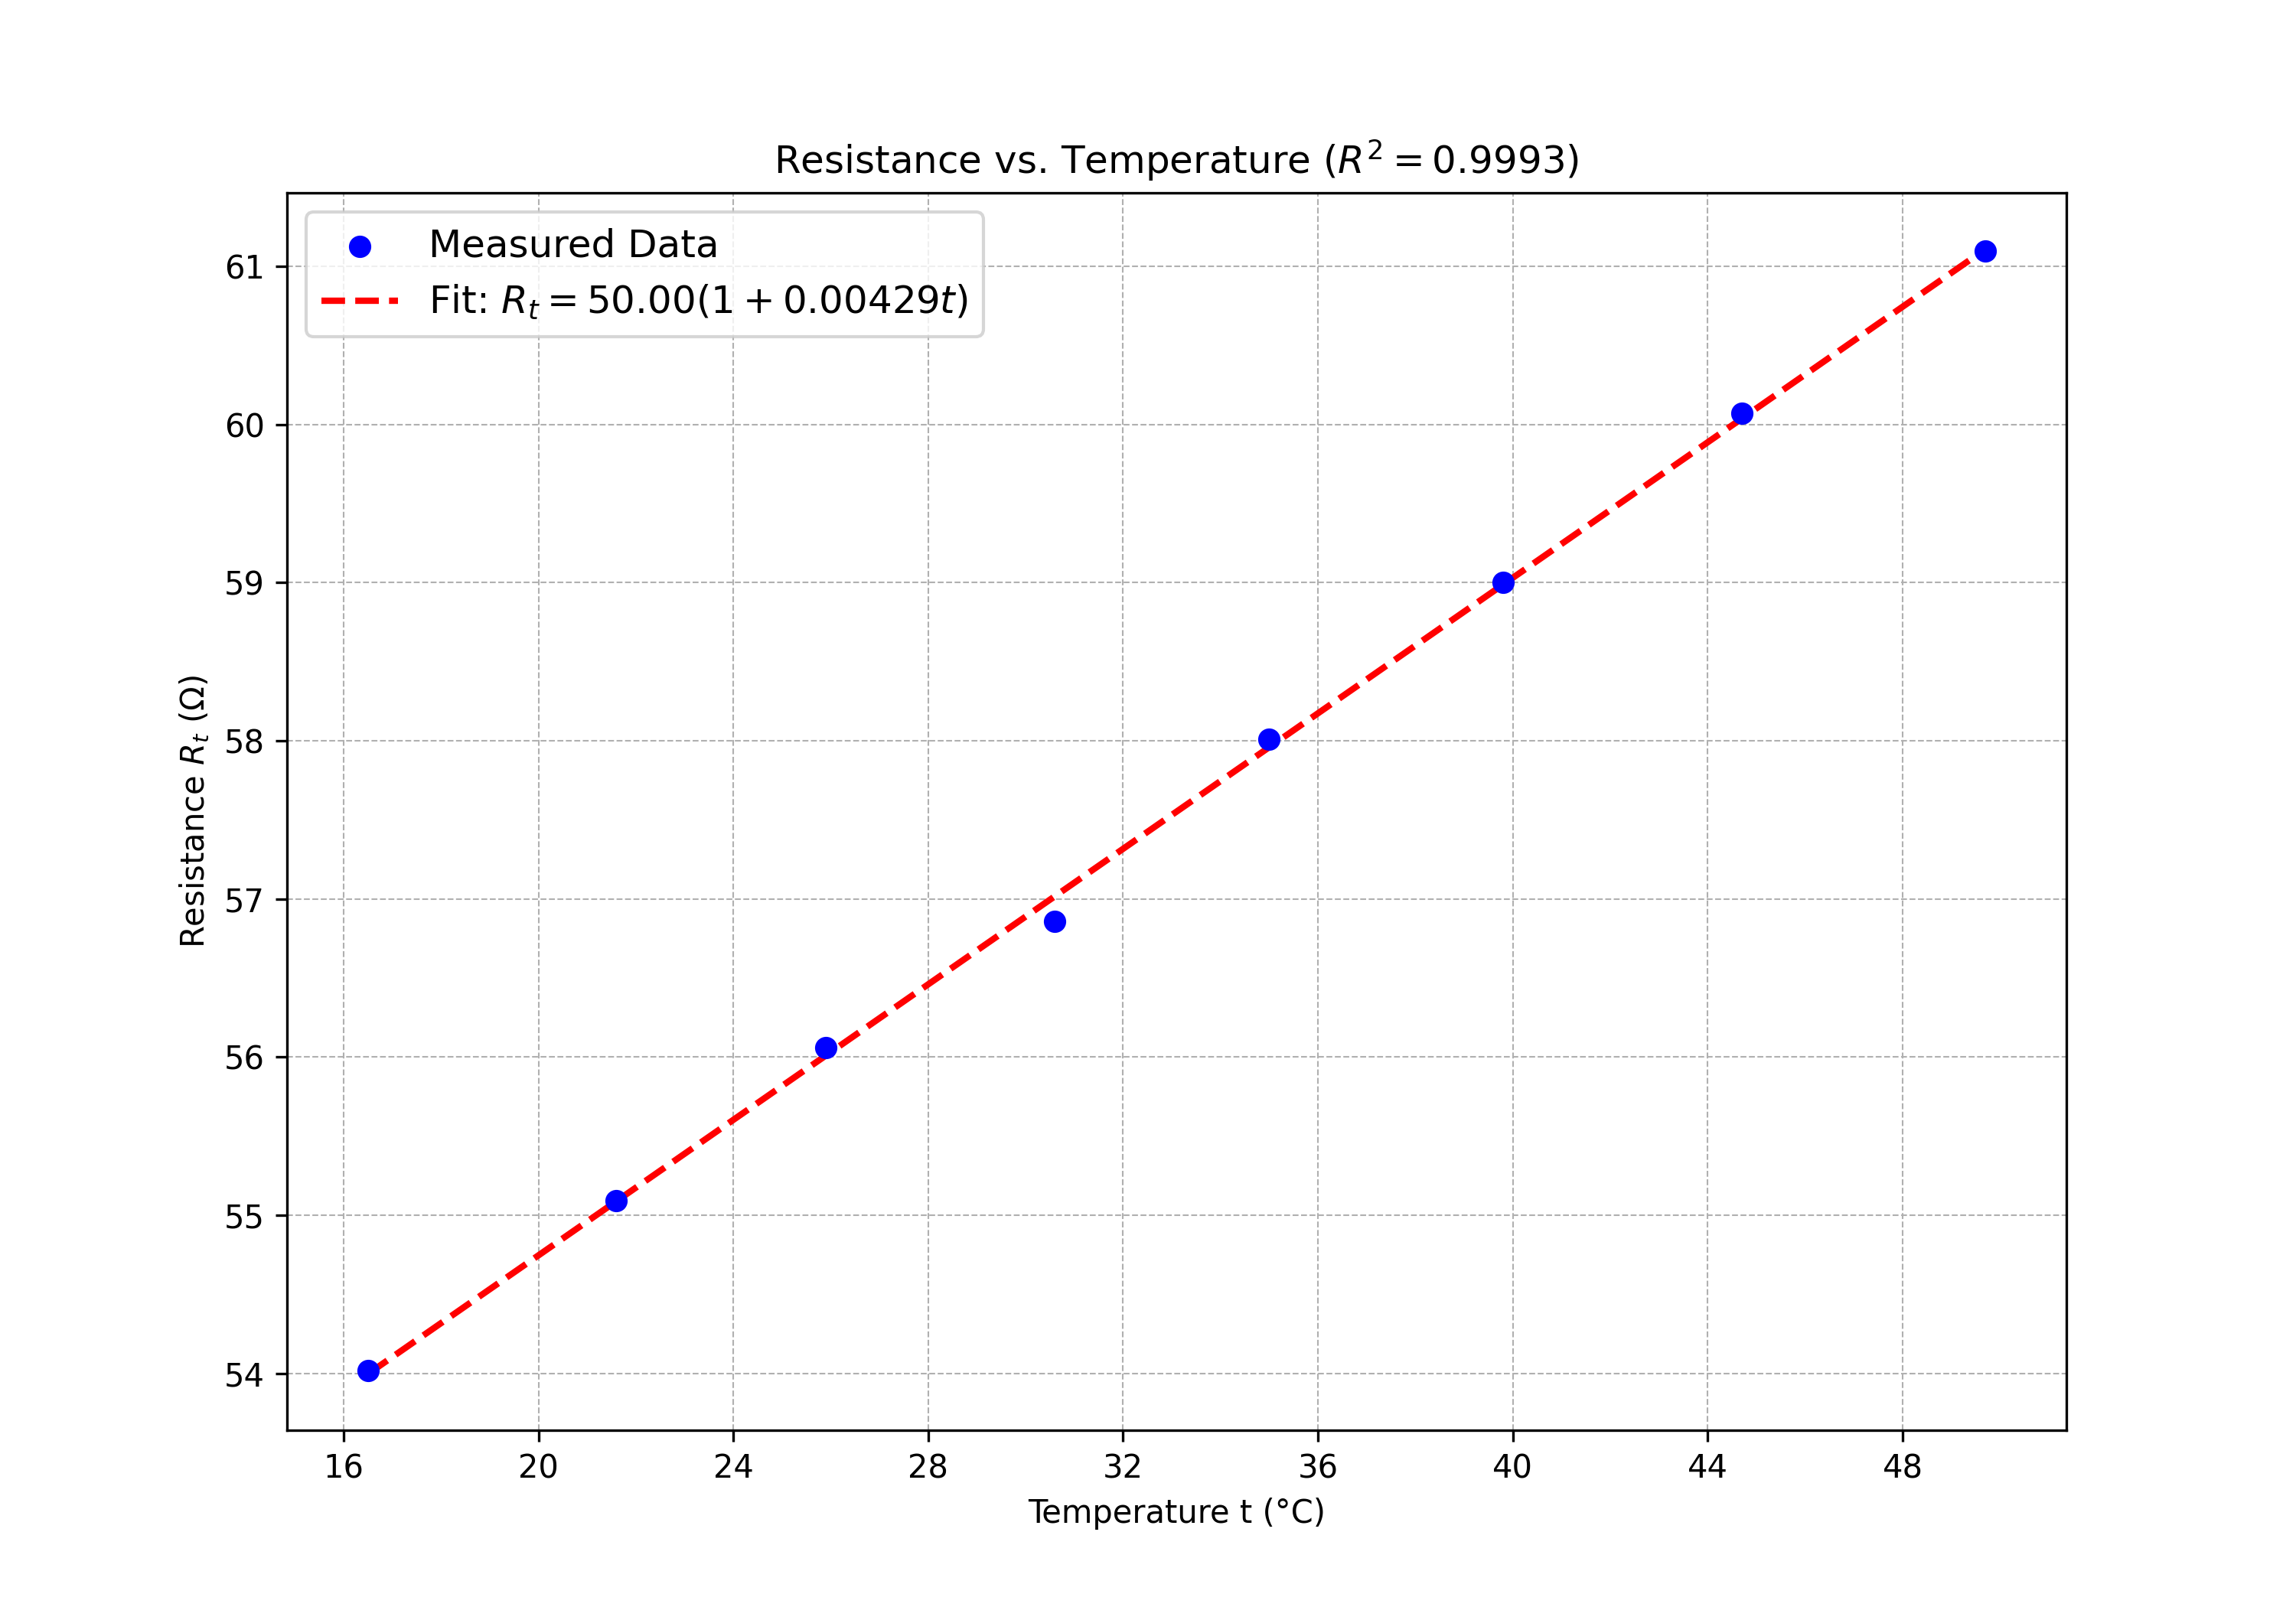
\includegraphics[width=0.9\textwidth]{figure/curve.png}
    \caption{平衡电桥测温度特性拟合曲线}
\end{figure}

计算相对误差为
\[
    \delta_{\mathrm{balance}}=\left|\frac{\alpha_{\mathrm{balance}}-\alpha_{\mathrm{theory}}}{\alpha_{\mathrm{theory}}}\right|=0.23\%
\]

    \myspace{2}
\subsection{误差分析}
    \xiaosi （运用测量误差、相对误差、不确定度等分析实验结果，20分）

    两个实验误差主要来源有以下几点：

    1.温度控制误差。实验装置通过设定温度加热来控制电阻温度，但是容易出现温度加热过头超过设定温度的情况，以及停止加热后电阻温度下降。电压值和温度值并非完全对应，存在一定误差。

    2.平衡电桥法控制电压为0V难以完全实现，需要忽略微小电压，导致读数存在误差。

    3.电阻调节误差。电阻箱设备老化，调节阻值时存在一定误差。

    4.电压表读数不稳，存在读数误差。
    \subsection{实验探讨}
    \xiaosi （对实验内容、现象和过程的小结，不超过100字，10分）

    通过本次实验，掌握了非平衡电桥和平衡电桥测量电阻温度特性的方法。实验结果表明平衡电桥法测量精度更高（误差0.23\%），而非平衡电桥法操作更简便但误差较大（5.0\%）。温度控制精度和电压测量准确性是影响实验结果的关键因素。
\section{思考题}

    \xiaosi （解答教材或讲义或老师布置的思考题，10分）

(1)简述非平衡电桥与平衡电桥之间的区别。

平衡电桥通过调节电阻使电桥输出电压为零，测量平衡状态下的电阻值；非平衡电桥则直接测量电桥在非平衡状态下的输出电压，通过电压与电阻变化的关系计算待测参数。平衡电桥测量精度高但操作复杂，非平衡电桥响应快适合动态测量。

(2)非平衡电桥在工程中有哪些应用？请举例说明。

非平衡电桥广泛应用于：
\begin{itemize}
    \item 温度测量：如热电偶温度计
    \item 应变测量：应变片测量材料形变
    \item 自动控制系统：如电子秤、压力传感器
    \item 成分分析：气体传感器检测浓度变化
\end{itemize}
其快速响应特性使其特别适合需要实时监测的场合。

\sihao\textbf{注意事项：}
\xiaosi
\begin{enumerate}
    \item 用PDF格式上传“实验报告”，文件名：学生姓名+学号+实验名称+周次。
    \item  “实验报告”必须递交在“学在浙大”的本课程的对应实验项目的“作业”模块内。
    \item  “实验报告”成绩必须在“浙江大学物理实验教学中心网站”-“选课系统”内查询。
    \item 教学评价必须在“浙江大学物理实验教学中心网站”-“选课系统”内进行，学生必须进行教学评价，才能看到实验报告成绩，教学评价必须在本次实验结束后 3 天内进行。
\end{enumerate}

\vspace{1cm}
\xiaosi\centering \textbf{浙江大学物理实验教学中心制}

\end{document}